\documentclass{extarticle}
\usepackage[a4paper, total={6.5in, 9.2in}]{geometry}
\usepackage[T1]{fontenc}
\usepackage{times}
\usepackage{verbatim}
\usepackage{graphicx}
\usepackage{amsmath}


\title{Sampling non-isotropic Gaussian random fields}
\author{Prashant Kumar}
\date{prashant721302@gmail.com}
\begin{document}
\maketitle
\texttt{RandField\_Matern.m} script  uses the following stationary non-isotropic Mat\'ern model 
\begin{align}
C_\Phi(\mathbf{x_1},\mathbf{x_2}) &= \sigma_c^2\dfrac{2^{1-\nu_c}}{\Gamma(\nu_c)}\left( 2\sqrt{\nu_c}\tilde{r}\right)^{\nu_c} K_{\nu_c}\left( 2\sqrt{\nu_c}\tilde{r}\right)\\
\tilde{r}  &= \sqrt{\dfrac{(x_1-x_2)^2}{\lambda^2_{cx}}+ \dfrac{(y_1-y_2)^2}{\lambda^2_{cy}}}\quad\text{with}\quad \mathbf{x_1} = (x_1,y_1),\mathbf{x_2} = (x_2,y_2).
\end{align}
where $\lambda_{cx}$ and $\lambda_{cy}$ are correlation lengths along x- and y-coordinates, respectively, $\nu_c$ is the smoothness of the random field and $\sigma^2_c$ is the marginal variance. Some examples of usage:

\vspace{1cm}
\texttt{>>[F]= RandField\_Matern(0.1,0.1,1,1,0,7,1)\% isotropic}\\
\centering
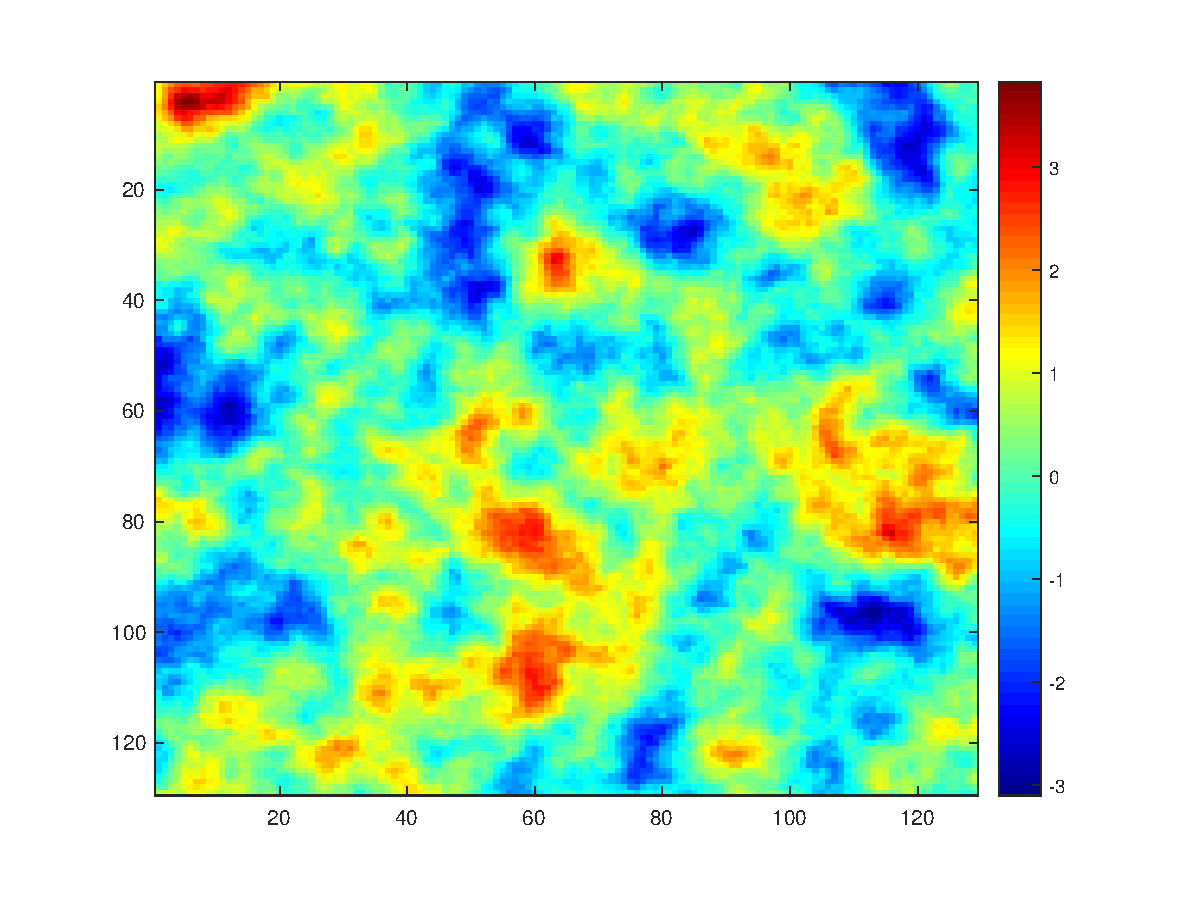
\includegraphics[scale=0.4]{f1.eps}\\
\texttt{>>[F]= RandField\_Matern(2,0.02,0.5,1,0,7,1)\% layering along x}\\
\centering
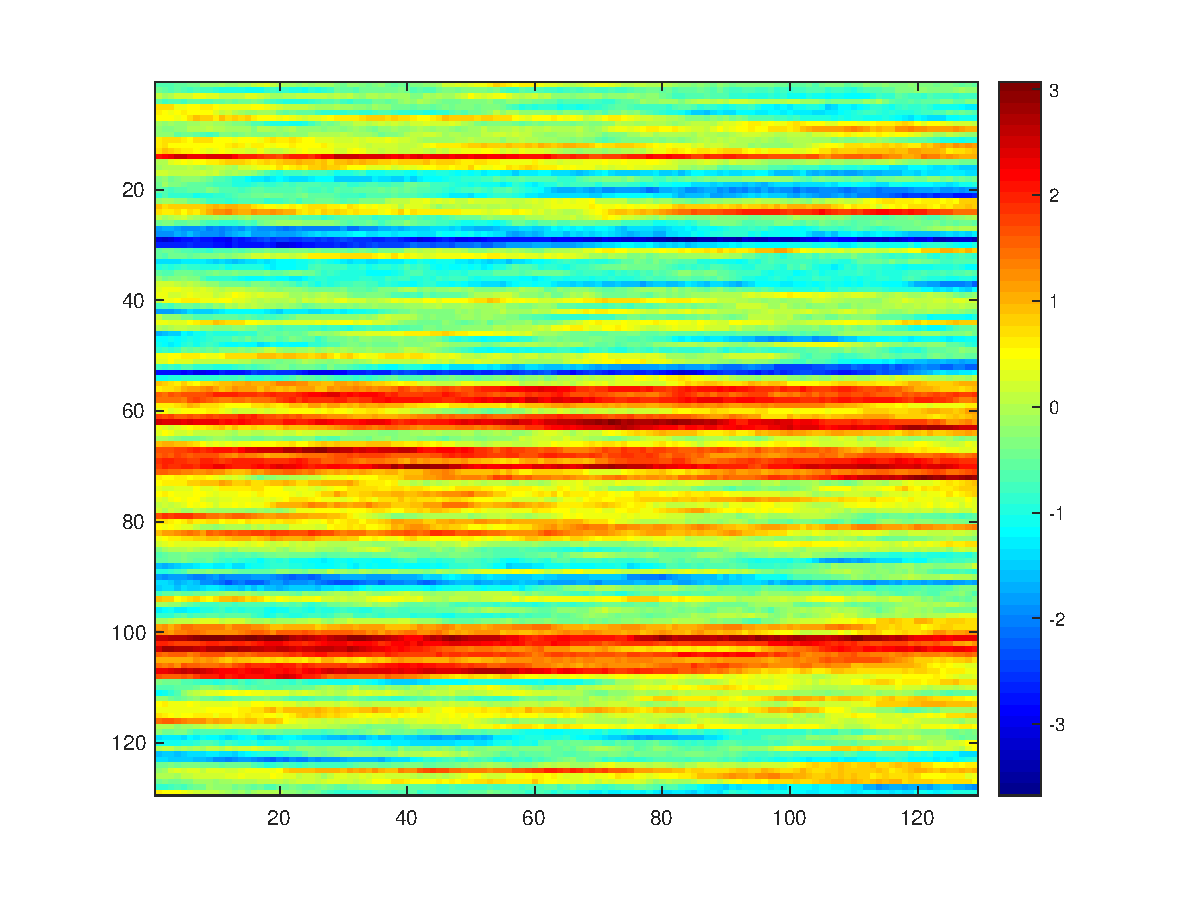
\includegraphics[scale=0.4]{f2.eps}\\
\texttt{>>[F]= RandField\_Matern(0.01,1,0.5,0.5,0,7,1) \% layering along y}\\
\centering
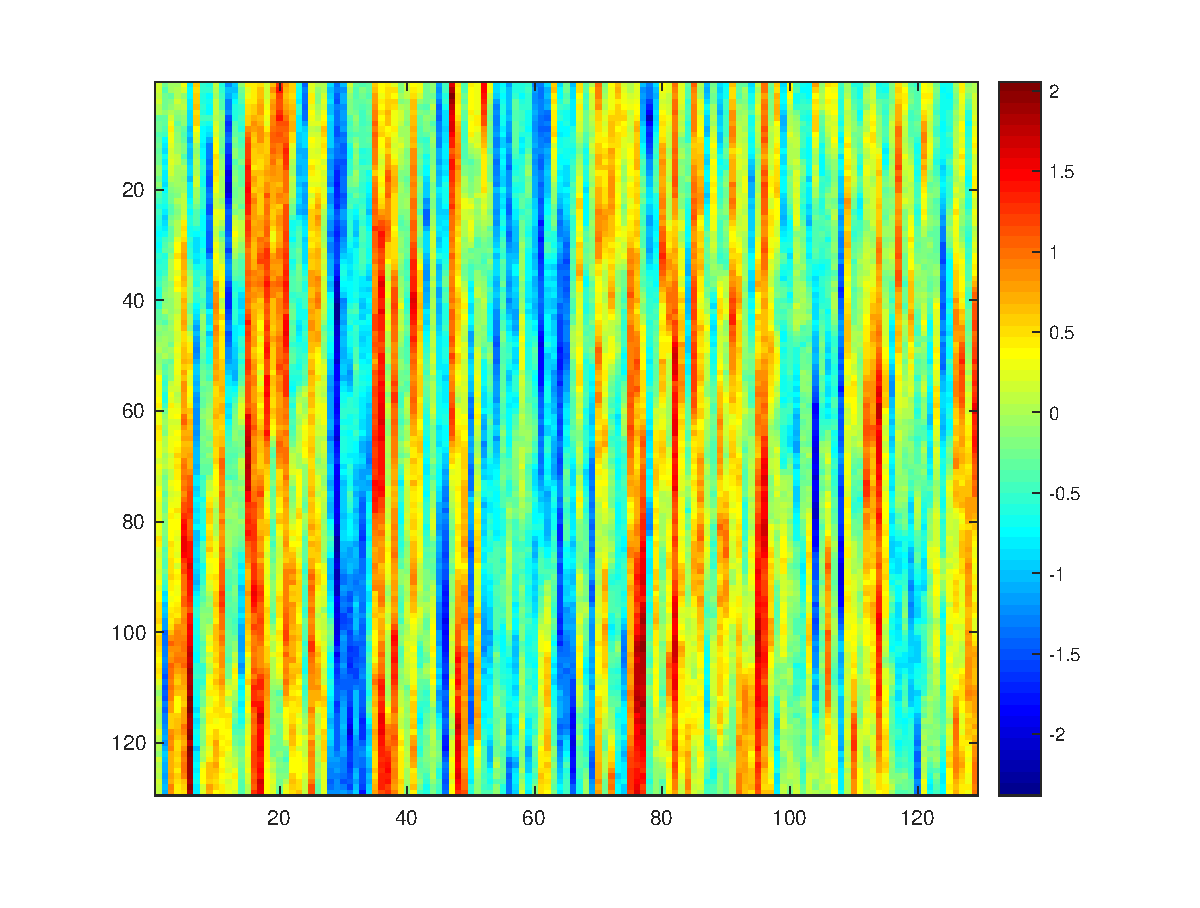
\includegraphics[scale=0.4]{f3.eps}\\
\vspace{1cm}

To generate tilted random fields, we use a modified version of the Mat\'ern covariance function, from \cite{kumarTransport},
\begin{equation}\label{aniso}
\begin{cases}
C_{\widetilde{\Phi}}(\mathbf{x_1},\mathbf{x_2}) = \sigma_c^2\dfrac{2^{1-\nu_c}}{\Gamma(\nu_c)}\left( 2\sqrt{\nu_c}\tilde{r}\right)^{\nu_c} K_{\nu_c}\left( 2\sqrt{\nu_c}\tilde{r}\right)\quad \mathbf{x_1},\mathbf{x_2}\in\mathcal{D},\\ 
\tilde{r} = \sqrt{\dfrac{(x_1'-x_2')^2}{\lambda^2_{cx}}+ \dfrac{(y_1'-y_2')^2}{\lambda^2_{cy}}},
\end{cases}
\end{equation}
where $C_{\widetilde{\Phi}}$ is a stationary covariance function depending on the parameter set ${\widetilde{\Phi}} = (\nu_c, \lambda_{cx}, \lambda_{cy}, \sigma_c^2,\theta)$ and $(x',y')$ corresponds to rotated coordinates by some angle $\theta$  in counterclockwise direction with respect to the horizontal axis, for e.g.
\begin{align}
x_1'  &= x_1\cos\theta - y_1\sin\theta,\nonumber\\
y_1'  &= x_1\sin\theta + y_1\cos\theta,\quad\text{with}\quad\mathbf{x_1} = (x_1,y_1)\nonumber.
\end{align}
The quantities $\lambda_{cx}$ and $\lambda_{cy}$ are correlation lengths along the x- and y-coordinates, respectively. The covariance function $C_{\widetilde{\Phi}}$ only differs from the isotropic covariance $C_\Phi$ defined in earlier in terms of the distance function $\tilde{r}$.\\
\vspace{1cm}

\texttt{>>[F]= RandField\_Matern(0.01,1,0.5,0.5,pi/4,7,1) \% aligned 45 degrees with x-axis}\\
\centering
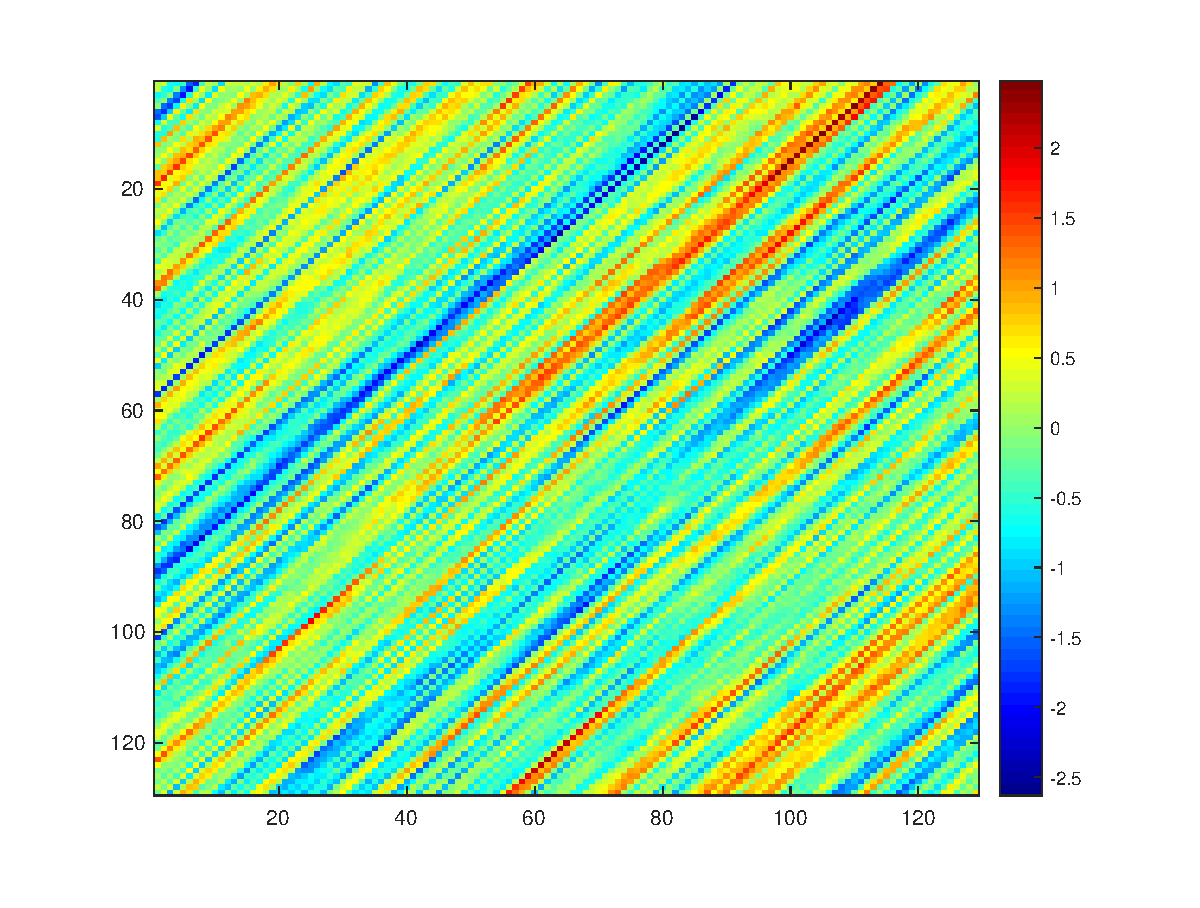
\includegraphics[scale=0.4]{f4.eps}\\


\begin{thebibliography}{10}
\bibitem{kumarTransport}
P.~Kumar, P.~Luo, F.~J. Gaspar, C.~W. Oosterlee, \textit{A multigrid multilevel
  Monte Carlo method for transport in the Darcy-Stokes system}, Journal of
  Computational Physics 371 (2018) 382 -- 408.  
\bibitem{RF4}
C.~{Dietrich}, G.~{Newsam}, \textit{Fast and exact simulation of stationary
  Gaussian processes through circulant embedding of the covariance matrix},
  SIAM J. Sci. Comput. 18 (1997) 1088--1107.
\bibitem{RF2}
A.~{Wood}, G.~{Chan}, \textit{Simulation of stationary Gaussian processes in
  $[0, 1]^d$}, Journal of Computational and Graphical Statistics 3 (1994)
  409--432.
\end{thebibliography}
\end{document}